\section{System Demo}
\kenny{This is a poster paper, not a demo paper! Try to restructure it as 
a poster paper. Check out some of the previous AAAI poster papers.}

The demonstration consists of two parts. The first showcases the association
knowledge base. The second illustrates the application of
the knowledge base in a recommendation system.

\kenny{The example in fig \ref{fig:gongli} doesn't have chinese translation.}
%\subsection{Association Knowledge Base}
Figure \ref{fig:gongli} demonstrates the result of querying the association knowledge base. The famous Chinese actress "Gong Li" is used as
a query concept. And all related concept for "Gong Li" are depicted in a clustered manner. When you type a concept into our system,
the system will return related concepts which is exhibited in a clustered manner. The closer the relationship, the shorter the distance between
the two concept in the figure. The more popular the related concept, the bigger the font used to display this concept.
%In order to evaluate the quality of our knowledge-base, we choose 20 keys for both general and person knowledge-base. Then we ask 10 persons to give a satisfactory score for each of the displayed terms. The score is between
%1-10. 1 means the term totally unrelated to the term mentioned in the query. 5 means the term relates to the term mentioned in the query but is not novel. 10 means the terms relates the term in the query and is very novel.

\begin{figure}[th]
\centering
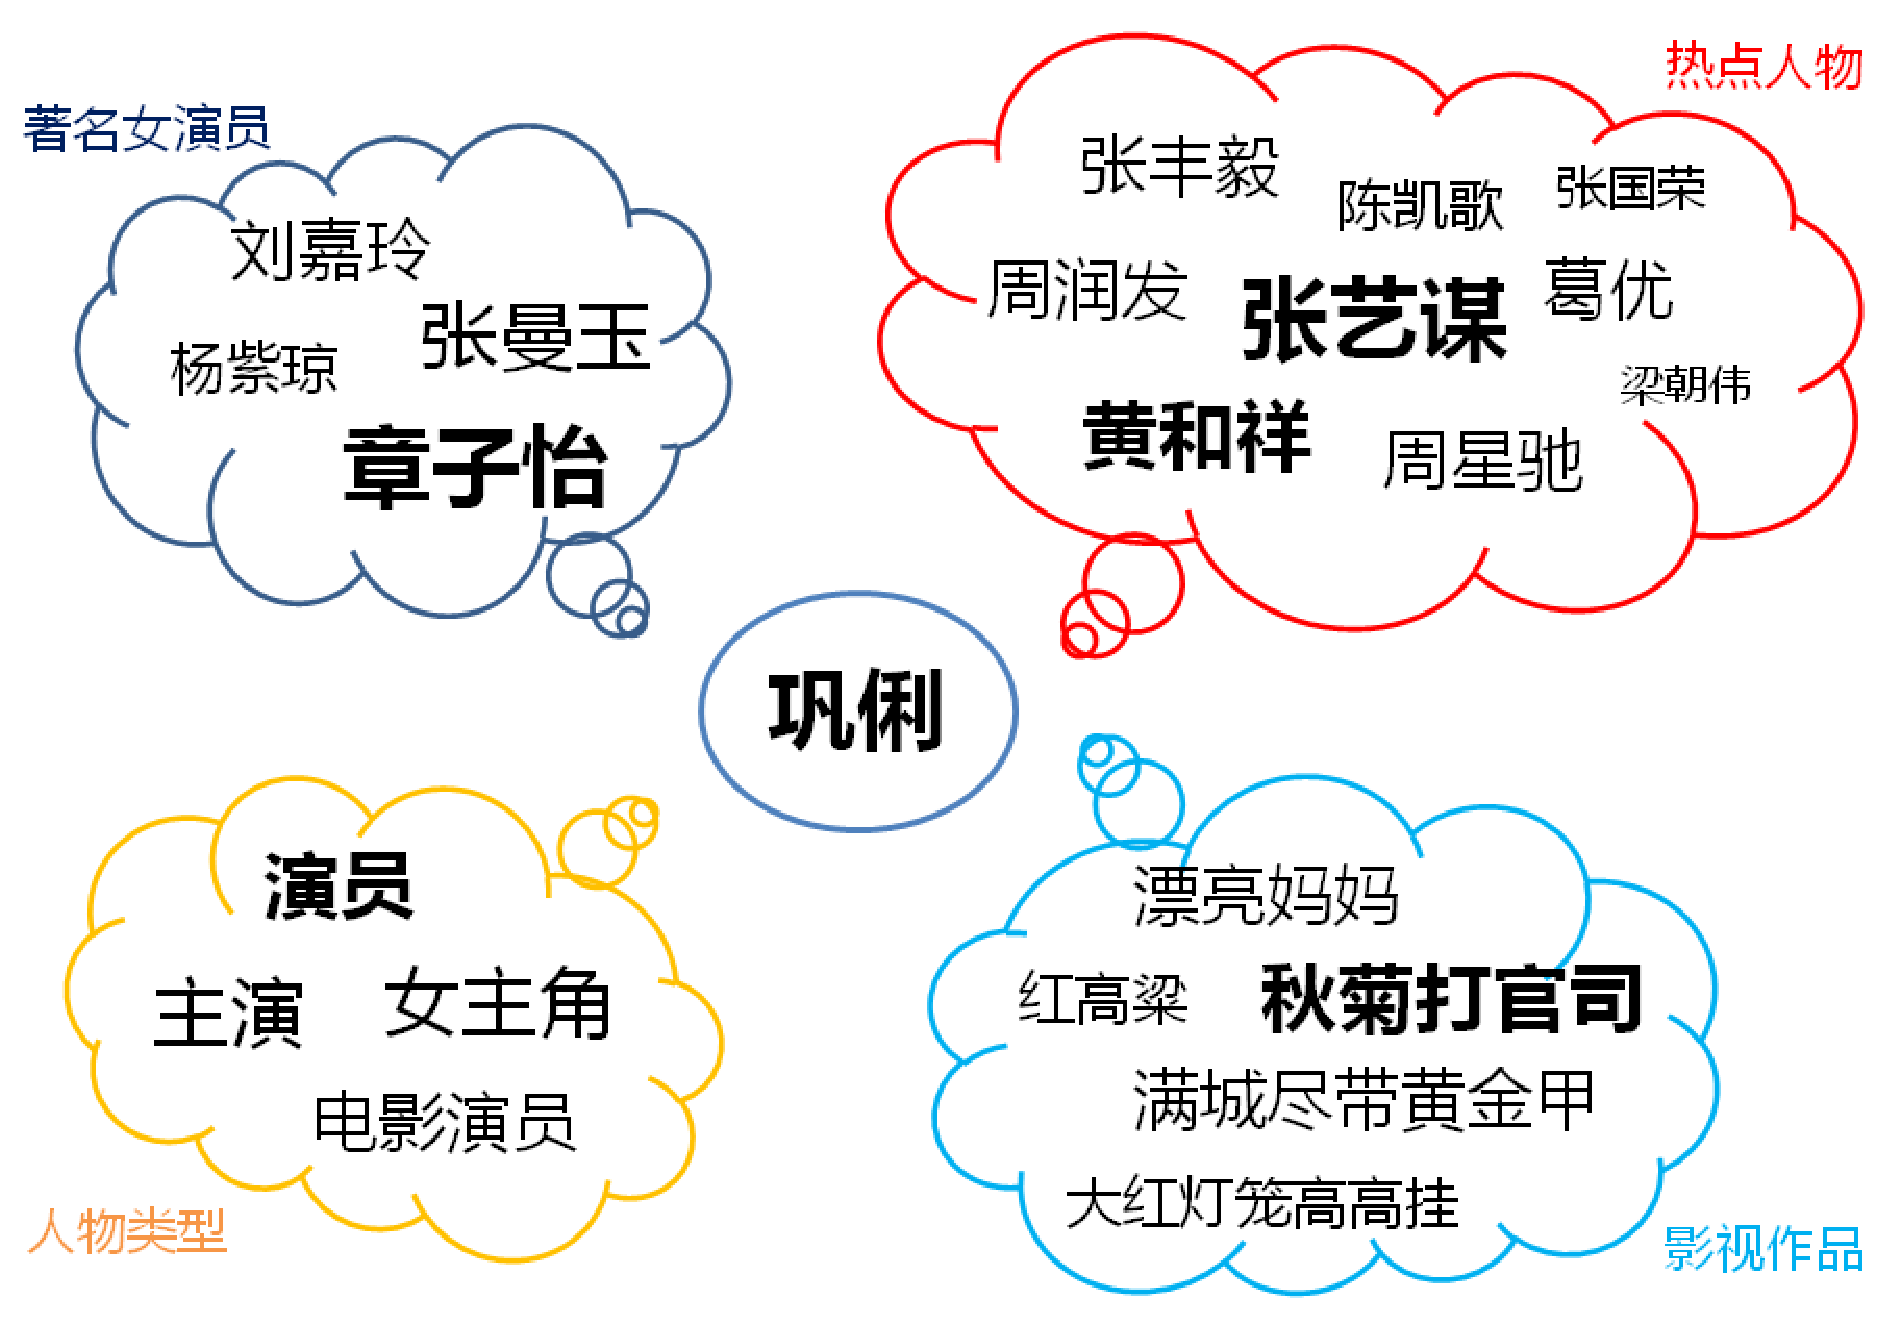
\epsfig{file=kb-cluster.eps,width=0.7\columnwidth}
\caption{Concepts Associated with Actress ``Gong Li'' and Their
Clusters.}
\label{fig:gongli}
\shrink
\end{figure}

%In addition to the graphic user interface, we also have an application programming interface(API) for the association knowledge-base. The API will return a ranked list of concepts which relate to the query concept.

%In figure \ref{fig:gongli}, the demonstration of our experimental
%result of general knowledge base is showed.
%And table \ref{table:1} illustrates the satisfactory score from students for both the general and the person knowledge base.
%\begin{figure}[!h]
%\small
%\centering
%\includegraphics[width=10cm]{demo1_2.eps}
%\caption{General Knowledge-Base Demonstration}
%\label{figure:2}
%\end{figure}

%\begin{table}
%\centering
%\caption{Satisfactory Score of the Experimental Result}
%\label{table:1}
%\begin{tabular}[h]{|c|c|c|c|}
%  \hline
  % after \\: \hline or \cline{col1-col2} \cline{col3-col4} ...
%  Knowledge Base & Highest Score & Lowest Score & Average Score \\
%  \hline
%  General Knowledge Base & 200 & 180 & 190 \\
%  \hline
%  Person Knwoledge Base & 200 & 165 & 170 \\
%  \hline
%\end{tabular}
%\end{table}

%\subsection{Application in Recommendation}
In this part of the demo, we showcase a prototype recommendation system
which uses both content-based recommendation and the more popular
collaborative filtering.
%The association network in recommendation system could not only improve the diversity and novelty of the recommendation result, but also make the recommendation explainable. When the association knowledge base is used
In content-based recommendation system, after the system generates a
user model from inputs (purchase history), association knowledge helps to
expand the user model and generate novel recommendations.
In collaborative filtering case, the knowledge base helps the system
relate two users who have latent connection or similarity.

\begin{figure}[th]
\centering
\epsfig{file=shoppingCartDemoAlter.eps,width=0.8\columnwidth}
\caption{\textcolor{red}{Association Based Collaborative Filtering}}
\label{fig:rec_result}
\shrink
\end{figure}

\begin{figure}[th]
\centering
\epsfig{file=compare.eps,width=0.9\columnwidth}
\caption{\textcolor{red}{Comparison Different Recommendation Algorithm}}
\label{fig:rec_compare}
\shrink
\end{figure}

\kenny{What are you trying to say with fig \ref{fig:rec_result}? There's no description at all. There's no description about fig \ref{fig:rec_compare} also.
You need keep this abstract in 2 pages. Remember this is a 2 page extended 
abstract. You need to keep everything simple but yet present an interesting
problem or an interesting solution.}


\textcolor{red}{Figure \ref{fig:rec_result}}

%illustrates the use of association in collaborative filtering recommendation system. At the first glance, $userA$ and $userB$ are unrelated because they have different purchase histories. When applying the association knowledge base, the latent relationship between $userA$ and $userB$ could be discovered. The CD and car cleaner are all related to the concepts ``car''
%and ``trip''. The tent and beer indicates a trip to camping, which in turn,
%also related to ``car.''
%Thus the latent relationship between $userA$ and $userB$ is discovered.
%Then the system recommends the CD to $userB$ and recommends a tent to $userA$.

%we can see the recommendation result of a user who watches a movie called ZhenhuanZhuan. Recommendation system gives a result of rings and clotheshorse. From the explanation of the recommendation result, we can see these two product are recommended because they're related to the movie content by a keywords.
